%% LyX 2.0.8.1 created this file.  For more info, see http://www.lyx.org/.
%% Do not edit unless you really know what you are doing.
\documentclass[english]{beamer}
\usepackage[T1]{fontenc}
\usepackage[utf8]{luainputenc}
\usepackage{verbatim}
\usepackage{amsmath}
\usepackage{amssymb}
\usepackage{graphicx}

\makeatletter
%%%%%%%%%%%%%%%%%%%%%%%%%%%%%% Textclass specific LaTeX commands.
 % this default might be overridden by plain title style
 \newcommand\makebeamertitle{\frame{\maketitle}}%
 \AtBeginDocument{
   \let\origtableofcontents=\tableofcontents
   \def\tableofcontents{\@ifnextchar[{\origtableofcontents}{\gobbletableofcontents}}
   \def\gobbletableofcontents#1{\origtableofcontents}
 }
 \long\def\lyxframe#1{\@lyxframe#1\@lyxframestop}%
 \def\@lyxframe{\@ifnextchar<{\@@lyxframe}{\@@lyxframe<*>}}%
 \def\@@lyxframe<#1>{\@ifnextchar[{\@@@lyxframe<#1>}{\@@@lyxframe<#1>[]}}
 \def\@@@lyxframe<#1>[{\@ifnextchar<{\@@@@@lyxframe<#1>[}{\@@@@lyxframe<#1>[<*>][}}
 \def\@@@@@lyxframe<#1>[#2]{\@ifnextchar[{\@@@@lyxframe<#1>[#2]}{\@@@@lyxframe<#1>[#2][]}}
 \long\def\@@@@lyxframe<#1>[#2][#3]#4\@lyxframestop#5\lyxframeend{%
   \frame<#1>[#2][#3]{\frametitle{#4}#5}}
 \def\lyxframeend{} % In case there is a superfluous frame end
 \newenvironment{centercolumns}{\begin{columns}[c]}{\end{columns}}

%%%%%%%%%%%%%%%%%%%%%%%%%%%%%% User specified LaTeX commands.
\usepackage{listings}
\usetheme{Warsaw}
% or ...
%\usetheme{Antibes}	% tree outline, neat
%\usetheme{JuanLesPins}	% like Antibes, with shading
%\usetheme{Bergen}	% outline on side
%\usetheme{Luebeck}	% like Warsaw, square sides
%\usetheme{Berkeley}	% interesting left bar outline
%\usetheme{Madrid}	% clean, nice.  7/12 page numbers
%\usetheme{Berlin}	% dots show slide number
%\usetheme{Malmoe}	% OK, plain, unshaded
%\usetheme{Boadilla}	% nice, white bg, no top bar
%\usetheme{Marburg}	% nice, outline on right
%\usetheme{boxes}	% ???
%\usetheme{Montpellier}	% tree outline on top, plainish white
%\usetheme{Copenhagen}	% like Warsaw
%\usetheme{PaloAlto}	% looks good
%\usetheme{Darmstadt}	% like Warsaw with circle outline
%\usetheme{Pittsburgh}
%\usetheme{default}
%\usetheme{Rochester}	% like boxy, unshaded warsaw
%\usetheme{Dresden}	% circle outline on top
%\usetheme{Singapore}	% purple gradient top
%\usetheme{Frankfurt}	% like Warsaw with circle outline on top
%\usetheme{Szeged}
%\usetheme{Goettingen}	% light purple right bar outline
%\usetheme{Warsaw}
%\usetheme{Hannover}	% like Goett with bar on left
%\usetheme{compatibility}
%\usetheme{Ilmenau}

\setbeamercovered{transparent}
% or whatever (possibly just delete it)

%\usecolortheme{seahorse}
%\usecolortheme{rose}

% seems to fix typewriter font in outline header:
\usepackage{ae,aecompl}

\makeatother

\usepackage{babel}
\begin{document}

\title{Preserving Type I error in rare allele GWAS}


\author{Dan Schlauch, PhD Candidate}


\institute{Department of Biostatistics\\
Harvard School of Public Health}


\date{\today}

\makebeamertitle


\pgfdeclareimage[height=0.5cm]{institution-logo}{institution-logo-filenameO}

\logo{\pgfuseimage{institution-logo}}

% RPD:  can't get this to work on any template.  not present in Warsaw any way, it seems

% hmm, problem seems to be that it isn't copied to the tmp dir, probably becuase it doesn't have the

% filename extension (which is tacked on by pgf it seems)

%\AtBeginSubsection[]{

%  \frame<beamer>{ 

%    \frametitle{Outline}   

%    \tableofcontents[currentsection,currentsubsection] 

%  }

%}

%\beamerdefaultoverlayspecification{<+->}


\lyxframeend{}\lyxframe{Outline}

\tableofcontents{}


\lyxframeend{}


\lyxframeend{}\section{Differential confounding for rare alleles}


\lyxframeend{}\subsection{Inflation due to stratification}


\lyxframeend{}\lyxframe{Rare allele association inflation}

\begin{center} 

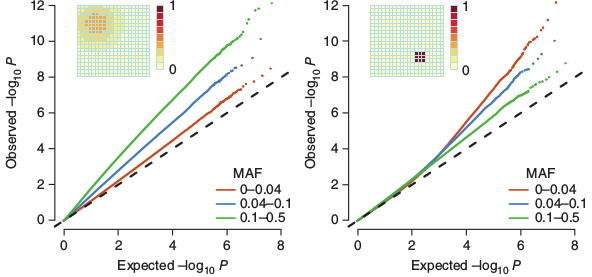
\includegraphics[width=0.6\paperwidth]{pasted1}\\
QQ plots of p-values separated by allele frequency. Comparing two
types of non-genetic risk distributions. {\textbf{Mathieson, Nature
Genetics 2012}}

 \end{center}


\lyxframeend{}


\lyxframeend{}\lyxframe{Rare allele association inflation}
\begin{block}
{Differential confounding by allele frequency}

The magnitude of confounding due to stratification is a function of
allele frequency and phenotypic distribution
\begin{itemize}
\item For a gradual phenotypic distribution.

\begin{itemize}
\item Greater inflation of \textbf{common} alleles
\end{itemize}
\item For a sharp phenotypic distribution

\begin{itemize}
\item Greater inflation of \textbf{rare} alleles
\end{itemize}
\end{itemize}
\end{block}

\lyxframeend{}


\lyxframeend{}\subsection{Problems with stratification correction}


\lyxframeend{}\lyxframe{Rare allele association inflation}

\begin{center} 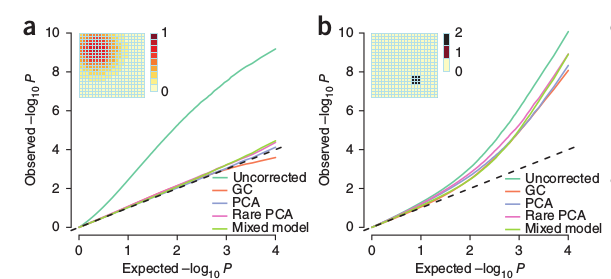
\includegraphics[width=0.6\paperwidth]{pasted2}

\textbf{Mathieson, Nature Genetics 2012}\foreignlanguage{english}{ \end{center}}

\selectlanguage{english}%
Existing methods for correction for population stratification do not
work for sharp phenotypes (and are particularly ineffective for rare
variants).


\lyxframeend{}


\lyxframeend{}\section{Why do we observe inflation?}


\lyxframeend{}\lyxframe{There are at least 3 problems}
\begin{enumerate}
\item Common stratification correction methods use linear functions to define
risk and do not distinguish a tree-like ancestry particularly well.

\begin{enumerate}
\item Need better estimates of genetic relatedness.
\end{enumerate}
\item Differential genotype/phenotype variances lead to scaling of null
test statistic distribution.

\begin{enumerate}
\item Need better estimates of test statistic overdispersion.
\end{enumerate}
\item Finite sample sizes yield overdispersion of association statistic.

\begin{enumerate}
\item Need improvements over use of asymptotic distributions.
\end{enumerate}
\end{enumerate}

\lyxframeend{}


\lyxframeend{}\lyxframe{Addressing fine-scale stratification}

\begin{block}{Common stratification correction approach}
\begin{itemize}   
\item Build a variance-covariance matrix between all samples using all variants and identify top axes of variation via PCA. (Eigenstrat)
\item Apply correction use the top  PCs.
\end{itemize}
\end{block}
\begin{block}{Limitations}
\begin{itemize} 
\item Assumes populations are linearly structured in space.
\item Inherently relies on common variants relative to rare variants.
\end{itemize}
\end{block}


\lyxframeend{}


\lyxframeend{}\lyxframe{Addressing fine-scale stratification}


\lyxframeend{}


\lyxframeend{}\subsection{Problems with the current methods of using NCS}


\lyxframeend{}\lyxframe{Typical MATLAB-NCS usage}

{\footnotesize{}\verbatiminput{thesispres-matlabexample.txt}}{\footnotesize \par}


\lyxframeend{}


\lyxframeend{}\lyxframe{My MATLAB-NCS experience}


\note[item]{talk about my work on Maciokas' visual cortex model in MATLAB}
\begin{block}
{}
\begin{itemize}
\item ``printf'' style model building is limited

\begin{itemize}
\item Easy to make errors
\item Small changes to model can require many changes
\end{itemize}
\item Saving models and then executing them is limiting

\begin{itemize}
\item Prevents strategies like GA search for models
\item Prevents encapsulation of an ``experiment as a script''
\end{itemize}
\item There is typically very little code reuse
\item MATLAB is not a particularly elegant text processing language
\item MATLAB support for general purpose libraries is weak
\end{itemize}
\end{block}

\lyxframeend{}


\lyxframeend{}\subsection{Design goals for a new approach to using NCS}


\lyxframeend{}\lyxframe{Design goals for a new approach to using NCS}
\begin{block}
{}
\begin{itemize}
\item <1->Allow very complex experiments with maximum clarity and minimum
effort
\item <2->Allow very simple experiments with minimum overhead
\item <3->A model is a script (there is no other reasonable way)
\item <4->Object oriented neural model design
\item <5->Integrated modeling, experimentation, analysis
\item <6->Container for standard, reusable component libraries.
\item <7->Free, and open source, from top to bottom
\item <8->Based on a language that is clean, good at text processing as
well as math, with extensive general purpose libraries
\item <9->Remote or local operation; make remote operation transparent
\item <10->Possible interactive use
\end{itemize}
\end{block}

\lyxframeend{}


\lyxframeend{}\section{Introduction to Brainlab}


\lyxframeend{}\subsection{Design issues}


\lyxframeend{}\lyxframe{Why Python?}
\begin{block}
{}
\begin{itemize}
\item Open source, free
\item Widely used and growing, active scientific community
\item Competitive array math package and plotting packages
\item Clean language design
\item Object oriented, dynamically typed, garbage collected, bytecode compiled
\item Efficient
\item Enforced indentation!
\end{itemize}
\end{block}

\lyxframeend{}


\lyxframeend{}\lyxframe{Brainlab implementation}
\begin{block}
{}
\begin{itemize}
\item <1->\texttt{COLUMN}, \texttt{LAYER}, \texttt{CELL}, \texttt{SYNAPSE}
are Python object classes
\item <2->These are \emph{nested} classes of \texttt{BRAIN} class
\item <3->\texttt{\_\_repr\_\_()} is overridden to output the \texttt{.in}
file representation
\item <4->NCS parameter names are dictionary keys
\item <5->Three modules:

\begin{itemize}
\item <5->brainlab.py: simulation environment, data analysis, graphing
\item <5->brain.py: model construction
\item <5->netplot.py: three dimensional display
\end{itemize}
\end{itemize}
\end{block}

\lyxframeend{}


\lyxframeend{}\lyxframe{netplot 3D module}


\lyxframeend{}


\lyxframeend{}\section{More complex examples}


\lyxframeend{}\subsection{My Ph.D. research}


\lyxframeend{}\lyxframe{My Ph.D. research}


\framesubtitle{Could a cortical microcircuit act as a functional unit for the memorization
of correlations of spatio-temporal spike trains?}
\begin{centercolumns}%{}


\column{6cm}
\begin{block}
{}
\begin{itemize}
\item Layer structured cortical microcircuit model
\item Two input cell groups

\begin{itemize}
\item Key
\item Data
\end{itemize}
\item Output cell group
\item Spatio-temporal spike trains as fundamental unit of information
\end{itemize}
\end{block}

\column{6cm}

\end{centercolumns}%{}

\lyxframeend{}


\lyxframeend{}\lyxframe{Stimulus patterns}



\begin{center}

\par\end{center}


\lyxframeend{}


\lyxframeend{}\lyxframe{My Ph.D. research: genetic model search}

\texttt{\tiny{}\verbatiminput{bigdemoga1.py}}{\tiny \par}


\lyxframeend{}


\lyxframeend{}\lyxframe{My Ph.D. research: genetic model search}

\texttt{\footnotesize{}\verbatiminput{bigdemoga2.py}}{\footnotesize \par}


\lyxframeend{}


\lyxframeend{}\lyxframe{My Ph.D. research: automated pattern matching}


\lyxframeend{}


\lyxframeend{}\subsection{An investigation into self-sustaining firing}


\lyxframeend{}\lyxframe{Phase space transitions in a recurrent network}


\begin{block}
{Dr. Doursat:}

``My goal is to explore bistability and other firing modes of the
network through a survey of parameter space (especially E/I to E/I
connections) and, from there, reveal what difference synaptic augmentation
(SA) and/or reciprocal connections can make (changes in phase space
landscape; easiness of phase transitions) when they are added to the
model.''

\end{block}

\lyxframeend{}


\lyxframeend{}\lyxframe{Setting up the experiment in Brainlab}
\begin{block}
{}
\begin{itemize}
\item Convert plain .in file into a script
\item Create experiment script
\item Create data analysis/graphing
\end{itemize}
\end{block}



\lyxframeend{}


\lyxframeend{}\section{Prospects}


\lyxframeend{}\lyxframe{Tighter integration with NCS}
\begin{block}
{Idea: eliminate NCS parsing module, and most of NCS' biological
knowledge}
\begin{itemize}
\item Simpler code; just a ``flat'' simulation engine that accepts GCList
\item Less redundancy of code and documentation
\item NCS would be more easily used with unstructured networks
\item Easier to add new features
\end{itemize}
\end{block}

\lyxframeend{}


\lyxframeend{}\lyxframe{Short-term enhancements to Brainlab}
\begin{block}
{}
\begin{itemize}
\item Some BRAIN.methods become brainlab functions
\item Data loading and report plotting standardized, expanded
\item Subdirectories for job execution (at least as an option)
\item Support for new queueing environments
\item Convenience functions for executing multiple jobs
\item Automated installation, configuration, testing
\item Expanded examples library
\end{itemize}
\end{block}

\lyxframeend{}


\lyxframeend{}\lyxframe{Use, so far}
\begin{block}
{}
\begin{itemize}
\item A colleague in our lab used an earlier version of Brainlab
\item I have made very extensive use of Brainlab in my own experiments
\item A colleague in our lab has recently begun using Brainlab in his experiments
\item Another lab is beginning to use NCS, and expressed interest in Brainlab
\end{itemize}
\end{block}

\lyxframeend{}


\lyxframeend{}\lyxframe{Acknowledgements}
\begin{block}
{Thanks to:}
\begin{itemize}
\item My committee
\item Dr. Harris, chair
\item Dr. Goodman, for the Brain Lab
\item Brain Lab colleagues
\end{itemize}
\end{block}

\lyxframeend{}
\end{document}
